%%%% Paramétrage du TD %%%%
\def\xxactivite{ \ifprof {Activation 2 -- Corrigé } \else  \ifcolle Colle \else Activation 2\fi \fi} % \normalsize \vspace{-.4cm}
\def\xxauteur{\textsl{Xavier Pessoles}}


\def\xxnumchapitre{Chapitre 1 \vspace{.2cm}}
\def\xxchapitre{\hspace{.12cm} Approche énergétique}

\def\xxcompetences{%
\vspace{-.5cm}
\footnotesize{
\textsl{%
\textbf{Savoirs et compétences :}\\
\vspace{-.2cm}
\begin{itemize}[label=\ding{112},font=\color{ocre}] 
\item Mod2.C18.SF1 : Déterminer l’énergie cinétique d’un solide, ou d’un ensemble de solides, dans son mouvement par rapport à un autre solide.
\item Res1.C1.SF1 : Proposer une démarche permettant la détermination de la loi de mouvement.
%\item Mod1.C5.SF2 : Déterminer la puissance des actions mécaniques extérieures à un solide ou à un ensemble de solides, dans son mouvement rapport à un autre solide.
%\item Mod1.C5.SF3 : Déterminer la puissance des actions mécaniques intérieures à un ensemble de solides.
\end{itemize}}}}


\def\xxtitreexo{Télécabine à stabilité accrue : le funitel}%Motorisation du moteur Haibike}
\def\xxsourceexo{\hspace{.2cm} \footnotesize{Mines Ponts PSI -- 2003}}

\def\xxfigures{
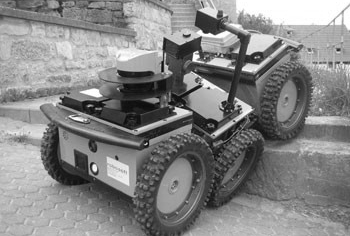
\includegraphics[width=.7\linewidth]{fig_00}
}%figues de la page de garde

\input{\repRel/Style/pagegarde_TD}
\setcounter{numques}{0}

\setlength{\columnseprule}{.1pt}

\pagestyle{fancy}
\thispagestyle{plain}


\vspace{5.2cm}

\def\columnseprulecolor{\color{ocre}}
\setlength{\columnseprule}{0.4pt} 

%%%%%%%%%%%%%%%%%%%%%%%

\setcounter{exo}{0}


\ifprof
%\begin{multicols}{2}
\else
\begin{multicols}{2}
\fi
\subsection*{Mise en situation}
\ifprof\else

Une télécabine est un système de transport de personnes permettant un changement d’altitude
important dans une zone d’accès difficile, généralement en montagne.

Les télécabines sont tractées par un câbles mis en mouvement par un ensemble motorisation. 
Afin de procéder à une évaluation de la puissance nécessaire à l’entrainement du câble, on
prendra comme modèle une ligne rectiligne supportée par 9 pylônes (voir figure au verso).


Le guidage des brins de câble est réalisé par des palonniers à galets fixés sur les pylônes,  pour lesquels le contact peut être modélisé par un appui avec frottement sec avec un coefficient de frottement $f = 0,03$. 2 brins permettent l'ascension de la cabine, 2 brins permettent la descente.
Cette donnée, associée à un calcul numérique des actions de contact des brins de câble sur les
palonniers, a permis une estimation à \SI{400}{kW} des pertes par frottement au niveau de ces
palonniers (puissance galiléenne des actions des palonniers sur les brins de câble).
L’action du vent sur une face d’une cabine est modélisable par une pression uniforme $p$ : $p=\dfrac{1}{2} \rho V_a^2$
avec $p$ en pascal, $\rho=\SI{1,3}{kg.m^{-3}}$ masse volumique de l’air, $V_a$ module de la vitesse relative de l’air par rapport à la cabine en m/s.



\fi
\begin{obj}
On étudiera la situation suivante (qui correspond à la situation la plus défavorable) : redémarrage de l’installation après un incident avec une accélération de \SI{0,15}{m.s^{-2}}. On se place à l’instant ou la vitesse de $\SI{7,2}{m.s^{-1}}$ va être atteinte, 8 cabines chargées de passagers sont en montée, 8 cabines vides sont en descente et un vent de vitesse $V_e = \SI{30}{m.s^{-1}}$ souffle parallèlement à la ligne dans le sens de la descente.
\end{obj}




\question{Déterminer l’énergie cinétique galiléenne, notée $E_{c_T}$, des 4 brins de câble, de l’ensemble
des cabines sur la ligne et de la motorisation, en fonction de $M_c$, $M_p$, $\mu$, $L$, $V$, $D_P$ et $I_M$.}
%L’application numérique donne pour la situation étudiée en négligeant la longueur de câble
%dans les gares : $E_{c_T}= \SI{6,7e6}{J}$ que l’on peut aussi écrire $E_{c_T}= \dfrac{1}{2}1,3\times 10^{5}V^2$ .}
\ifprof\begin{corrige} ~\\
\begin{itemize}
\item Énergie cinétique des 4 brins de câbles : $\ec{\text{cables}}{0} = \dfrac{1}{2}4 L \mu V^2$.
\item Énergie cinétique des 8 cabines montantes : $ \ec{{C_m}}{0} = \dfrac{1}{2}8  \left(M_c +  M_p\right) V^2$.
\item Énergie cinétique des 8 cabines descendantes : $\ec{{C_d}}{0} = \dfrac{1}{2}8  M_c V^2$.
\item Énergie cinétique de la motorisation : $\ec{\text{M}}{0} = \dfrac{1}{2}I_M  \omega_M^2$.
\end{itemize}

On a par ailleurs  $V=\omega_M \cdot \dfrac{D_p}{2}$.

On a donc $\ec{\Sigma}{0}= \dfrac{1}{2}\left(4 L \mu + 16 M_c + 8 M_p  + I_M\dfrac{4}{D_p^2}\right)V^2$.

On a donc $M_{\text{eq}}=4 L \mu + 16 M_c + 8 M_p  + I_M\dfrac{4}{D_p^2} = 4\times 1669 \times 8,47 + 16 \times 2500  + 8 \times 2080  + 575 \times 10^3 \dfrac{4}{16} = \SI{256936}{kg}$ et $\ec{\Sigma}{0}=\SI{6,7}{MJ}$.

\end{corrige}\else\fi


\question{Déterminer la puissance galiléenne, notée $P_p$, des actions de pesanteur sur l’installation en
fonction de $M_p$, $V$, $h$, $g$ et $L$. %L’application numérique donne pour la situation étudiée :
%$P_p = \SI{-3,6e5}{W}$.
}
\ifprof\begin{corrige} ~\\

Les puissances de la pesanteur sur les cabines montantes s'exprime ainsi : 

$\pext{\text{pes}}{C_m}{0} = \torseurstat{T}{\text{pes}}{C_m} \otimes \torseurcin{V}{C_m}{0}$
$ = 8 \torseurl{-\left(M_c+M_p\right)g \vect{z}}{\vect{0}}{G_c} \otimes \torseurl{\vect{0}}{V\vect{i}}{G_c}	$

$ = -8\left(M_c+M_p\right)gV\vect{z} \cdot \vect{i}$
$ = -8\left(M_c+M_p\right)gV \sin \alpha$.


Les puissances de la pesanteur sur les cabines descendantes s'exprime ainsi : 

$\pext{\text{pes}}{C_d}{0} = \torseurstat{T}{\text{pes}}{C_d} \otimes \torseurcin{V}{C_d}{0}$
$ = 8 \torseurl{-M_c g \vect{z}}{\vect{0}}{G_c} \otimes \torseurl{\vect{0}}{-V\vect{i}}{G_c}	$
$ = 8M_cgV\vect{z} \cdot \vect{i}$

$ = 8M_c gV \sin \alpha$.

Remarque : la puissance de la pesanteur sur le câble sont opposées pour la partie montante et la partie descendante.


Ainsi, $\pext{\text{pes}}{C_d+C_m}{0}=8M_c gV \sin \alpha -8\left(M_c+M_p\right)gV \sin \alpha$ 
$=-8M_pgV \sin \alpha$
$=\SI{-359289}{W}$.

\end{corrige}\else\fi


\question{Après avoir évalué la vitesse relative et l’action du vent sur une cabine en montée et une
cabine en descente, déterminer la puissance galiléenne, notée $P_v$ des actions du vent sur
l’ensemble des cabines en fonction de $\rho$, $S_f$, $V$, $V_e$ et $\alpha = \arcsin(h/L)$. %L’application
%numérique donne pour la situation étudiée : $P_v = \SI{- 2,2e5}{W}$.
}
\ifprof\begin{corrige}

%\textbf{Pour moi, le modèle pour l'action mécanique du vent n'est pas clair. On ne sait pas bien si l'effort est suivant $\vect{y}$ ou $\vect{i}$ Prenons .}
Le vent va dans le sens de la descente.  En montée, 
$\vectv{G_c}{\text{vent}}{C_m}=\vectv{G_c}{\text{vent}}{0}-\vectv{G_c}{C_m}{0}$ $=-V_e\vect{i} - V\vect{i}$.

En descente, 
$\vectv{G_c}{\text{vent}}{C_d}=\vectv{G_c}{\text{vent}}{0}-\vectv{G_c}{C_d}{0}$ $=-V_e\vect{i} + V\vect{i}$.

Les puissances du vent  sur les cabines montantes s'expriment ainsi : 
$p = \dfrac{1}{2}\rho V_a^2 = \dfrac{1}{2}\rho \left(-V-V_e\right)^2 $
$\pext{\text{vent}}{C_m}{0} = \torseurstat{T}{\text{vent}}{C_m} \otimes \torseurcin{V}{C_m}{0}$
$ = 8 \torseurl{-pS_f\vect{y}}{\vect{0}}{G_c} \otimes \torseurl{\vect{0}}{V\vect{i}}{G_c}	$
$ = -8S_fV\dfrac{1}{2}\rho \left(V+V_e\right)^2 \cos\alpha$.


Les puissances du vent  sur les cabines montantes s'expriment ainsi : 
$p = \dfrac{1}{2}\rho V_a^2 = \dfrac{1}{2}\rho \left(V-V_e\right)^2 $
$\pext{\text{vent}}{C_m}{0} = \torseurstat{T}{\text{vent}}{C_m} \otimes \torseurcin{V}{C_m}{0}$
$ = 8 \torseurl{-pS_f\vect{y}}{\vect{0}}{G_c} \otimes \torseurl{\vect{0}}{-V\vect{i}}{G_c}	$
$ =8S_fV\dfrac{1}{2}\rho \left(V-V_e\right)^2 \cos\alpha$.

Au final, $\pext{\text{vent}}{C_m+C_d}{0} =8S_fV\dfrac{1}{2}\rho \left(\left(V-V_e\right)^2- \left(V+V_e\right)^2\right)\cos\alpha$ $=8S_fV\dfrac{1}{2}\rho\left( -4VV_e\right)\cos\alpha$

$=-16S_f \rho V^2 V_e\cos\alpha$. On a donc 
%$ = -8\left(M_c+M_p\right)gV\vect{z} \cdot \vect{i}$
%$ = -8\left(M_c+M_p\right)gV \sin \alpha$.
$\pext{\text{vent}}{C_m+C_d}{0} = \SI{-218677}{W} $
\end{corrige}\else\fi


\question{En déduire une estimation de la puissance galiléenne nécessaire, notée $P_T$ pour
l’entrainement de la ligne entre les gares dans la situation étudiée. La puissance
effectivement installée par le constructeur est de \SI{1560}{kW}, commentez vos résultats par
rapport à cette valeur.}
\ifprof\begin{corrige}
On applique le théorème de l'énergie cinétique :

$\dfrac{\dd \ec{\Sigma}{0}}{\dd t} =\pext{\text{vent}}{C_m+C_d}{0} + \pext{\text{pes}}{C_m+C_d}{0} + \pext{\text{frottement}}{\Sigma}{0}+ \pext{\text{moteur}}{\Sigma}{0}$.

On a donc, en régime permanent : 
$0 = -229672-359289-400 000 +P_T $ $ P_T= 218677 + 359289 + 400 000 = \SI{977966}{W} \simeq \SI{1000}{kW}$.

En tenant compte de l'accélération, on a $P_T = \SI{1000}{kW}+  M_{\text{eq}} V\dot{V} =  \SI{1000}{kW}+  M_{\text{eq}} 7,2 \cdot 0,15 \simeq \SI{1266}{kW}$. 

Le surplus de puissance est nécessaire en cas de situation plus défavorable (plus de vent, dépassement du nombre de passagers...). 
\end{corrige}\else\fi

\ifprof
\else

Sur la ligne, les cabines se déplacent à $V = \SI{7,2}{m.s^{-1}}$. En gare, pour permettre l’embarquement et le
débarquement des passagers, la vitesse maximum de la cabine doit être de $v_0 = \SI{0.3}{m.s^{-1}}$.
Lors de leur circulation en gare, les cabines sont donc libérées des brins de câble,.% supportées et
%guidées par 4 galets sur deux rails parallèles. Elles sont entrainées par des trains de pneus
%constitués de roues de \SI{400}{mm} de diamètre, d’axe fixe, qui roulent sur un patin lié à la suspente
%articulée de la cabine.
%Dans une première analyse, 
On envisagera une accélération constante des cabines de $a=\SI{1.3}{m.s^{-2}}$.
%La% zone rectiligne de lancement %(secteur F) 
%comporte 45 roues pneumatiques. 
%Les roues du train
%de pneus sont reliées cinématiquement par des poulies-courroies qui assurent des rapports de
%réduction « $k_i$ » entre deux roues successives. %(voir dessin Fig. 8a : lanceur )
%L’entraînement de la roue la plus rapide (celle située en sortie de gare, roue n°45) est réalisé par
%la « poulie de guidage-déviation » du brin de câble en sortie de gare. Une chaîne cinématique
%assure cet entraînement.% (voir Fig. 3 : Photo Gare et Fig. 1 Ligne totale).
%Cette chaîne cinématique est constituée d’un mécanisme poulie-courroie et d’un multiplicateur de
%vitesse dont l’arbre d’entrée est directement entraîné par l’axe de la poulie de guidage-déviation.
%Cette poulie a un diamètre de \SI{4}{m}. On notera $K$ le rapport de multiplication de cette chaîne
%cinématique : K= w roue rapide45/ w poulie guidage déviation
%La zone de freinage (secteur A) est symétrique de la zone de lancement.
\fi
\question{Quelle est alors la durée $t$ de la phase d’accélération ? Exprimer la longueur $x$ (en mètre)
de la zone rectiligne en fonction de $a$ , $v_0$, $t$ et $V$. Pour que l’accélération de $\SI{1,3}{m.s^{-2}}$
permette le lancement des cabines de $v_0 = \SI{0,3}{m.s^{-1}}$ à $V = \SI{7,2}{m.s^{-1}}$, l’application numérique
donne environ : $x =\SI{20}{m}$.}
\ifprof\begin{corrige} ~\\

\begin{minipage}[c]{.4\linewidth}
\begin{center}
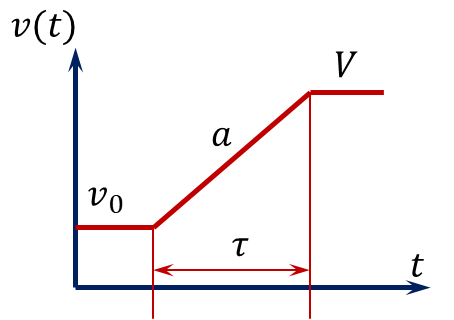
\includegraphics[width=0.95\textwidth]{cor_01}
\end{center}
\end{minipage} \hfill
\begin{minipage}[c]{.5\linewidth}

On a $v(t)=at+k$. Par ailleurs, $v(t_2)=V=at_2+k$ et $v(t_1)=v_0=at_1+k$. On a donc $V-v_0 =  a\tau $ soit $\tau = \dfrac{V-v_0}{a} = \dfrac{6,9}{1,3} =\SI{5,3}{s}$.


La distance parcourue pendant la durée $\tau$ correspond à l'intégrale de la vitesse soir à l'aire sous la courbe.
On a donc $x=\tau \cdot\dfrac{1}{2}\left(V+v_0\right)=5,3\times 0,5\times 7,5 = \SI{19,875}{m}$.
\end{minipage}
\end{corrige}\else\fi

\ifcolle
\else
\ifprof
\else
\noindent \footnotesize
\begin{tabular}{|p{\linewidth}|}
\hline
\begin{enumerate}
\item  $\ec{\Sigma}{0}= \dfrac{1}{2}\left(4 L \mu + 16 M_c + 8 M_p  + I_M\dfrac{4}{D_p^2}\right)V^2 \simeq \SI{6,7}{MJ}$.
\item $\pext{\text{pes}}{C_d+C_m}{0}=-8M_pgV \sin \alpha =\SI{-359289}{W}$.
\item $\pext{\text{vent}}{C_m+C_d}{0} =-16S_f \rho V^2 V_e\cos\alpha = \SI{-218677}{W} $.
\item $P_T = \SI{1266}{kW}$.
\item $\tau = \dfrac{V-v_0}{a} = \SI{5,3}{s}$ et $x=\tau \cdot\dfrac{1}{2}\left(V+v_0\right)= \SI{19,875}{m}$.
\end{enumerate} \\
\hline
\end{tabular}
\fi\fi
\normalsize


\ifprof
%\end{multicols}
\else
\end{multicols}
\fi


\ifprof
\else

\begin{center}
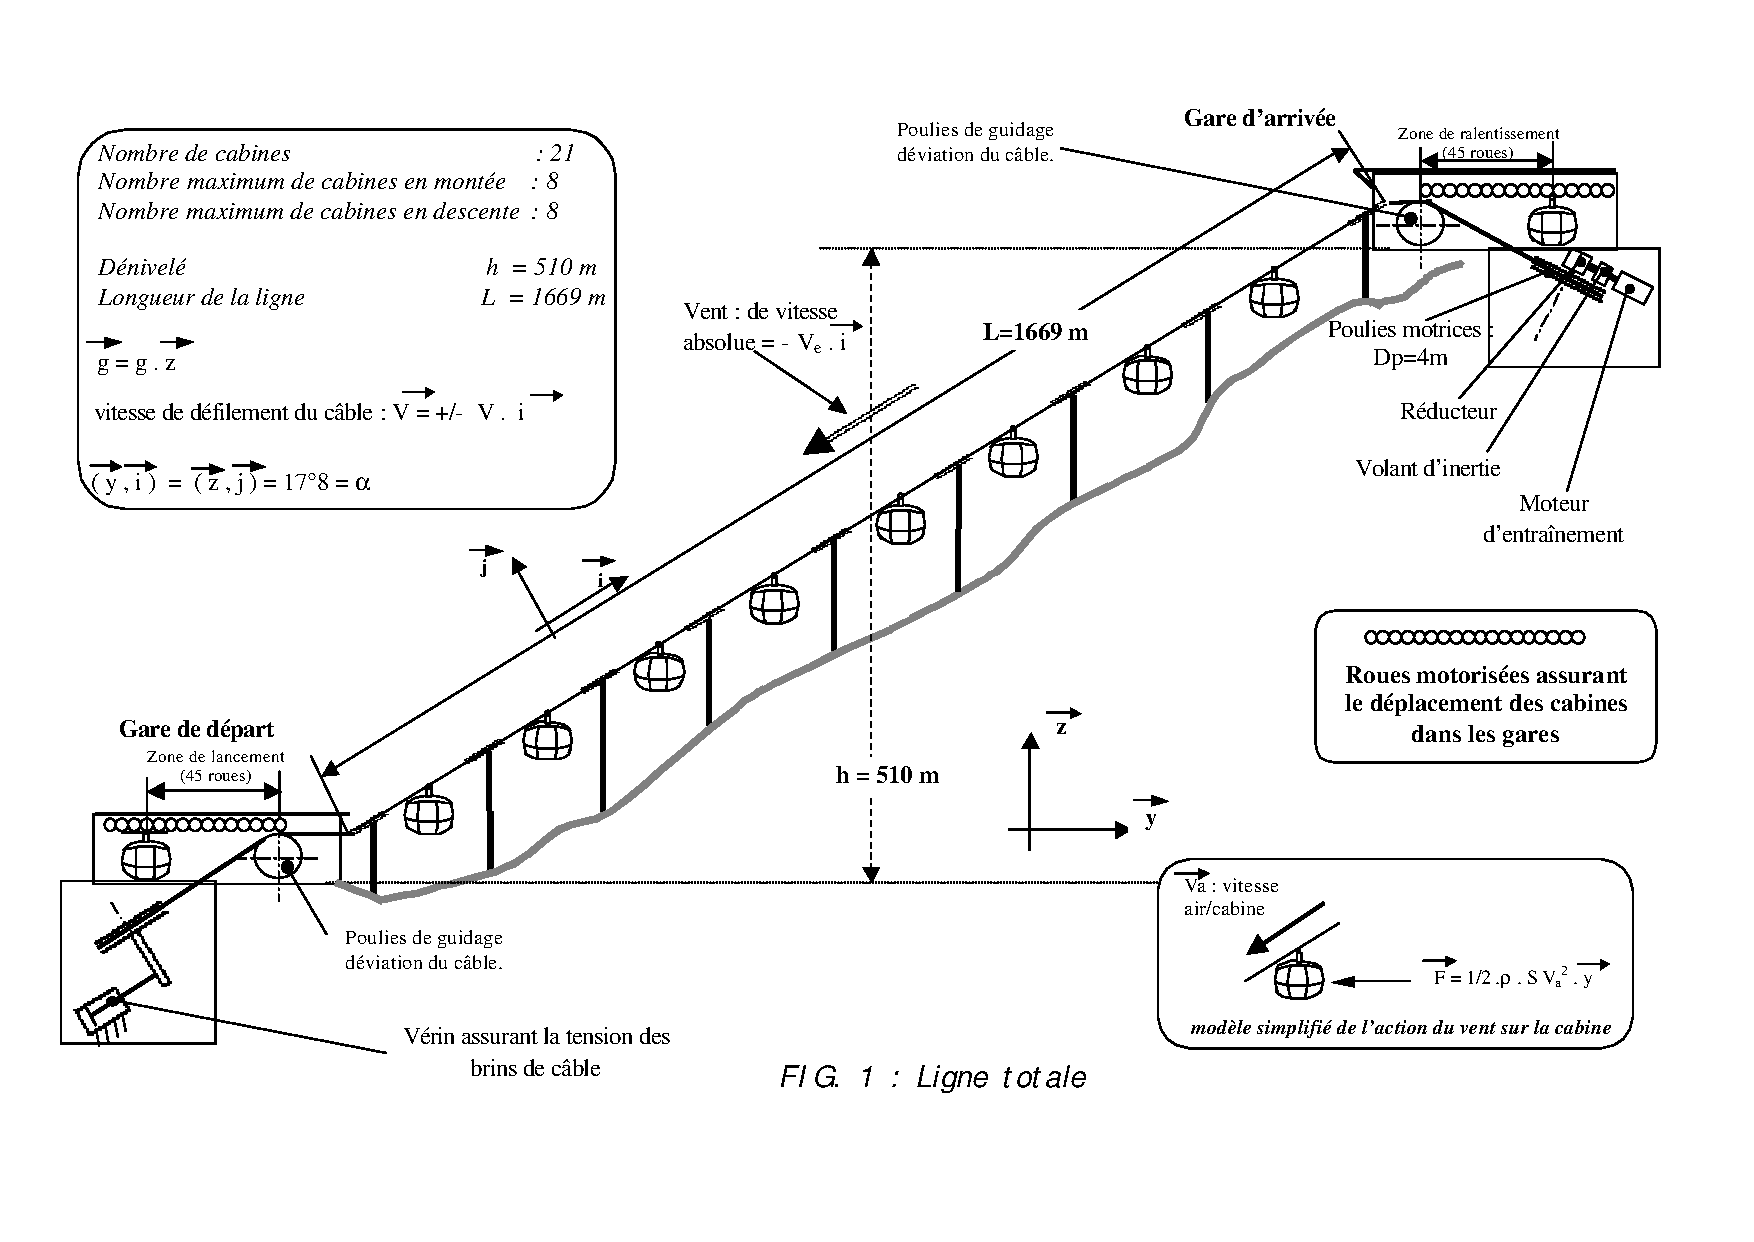
\includegraphics[width=0.9\textwidth]{fig_01.pdf}
\end{center}

\begin{center}
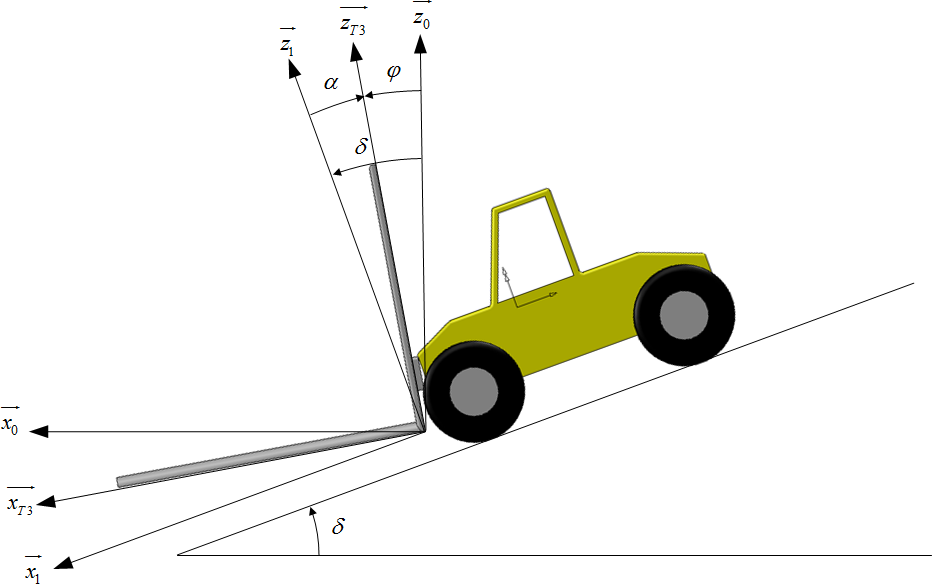
\includegraphics[width=0.9\textwidth]{fig_02.png}
\end{center}
\fi